\documentclass[varwidth,convert={density=500,size=1080x800,outext=.png}]{standalone}
\usepackage{mathtools}
\usepackage{graphicx}
\usepackage{bm}
\usepackage{color}
\usepackage[dvipsnames,table]{xcolor}
\usepackage{tikz}
\usepackage{stanli}
\usepackage{verbatim}
\usepackage{tikz}
\usetikzlibrary{shapes,calc,through,3d,patterns}
\usetikzlibrary{decorations.pathreplacing}
\usepackage{pgfplots}
\usepackage{siunitx} % For formatting numbers
\usepackage{hyperref}
\hypersetup{colorlinks=true,linkcolor=darkred}
\usepackage{multicol}
\usepackage[absolute,overlay,]{textpos}
\usepackage{pgfplots}
\pgfplotsset{width=10cm,compat=1.9}
\usepackage{subcaption}
\usepackage{multirow}
\usepackage{bbding}
\usepackage{arydshln}
\usepackage{mathtools}
\usepackage{tcolorbox}

\usepackage[dvipsnames]{xcolor}

\begin{document}
  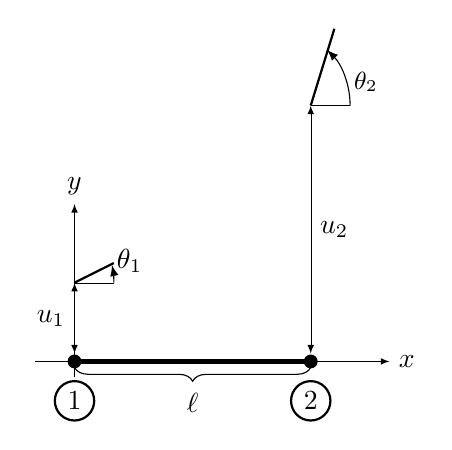
\begin{tikzpicture}[scale=1]
        % Define points
        \coordinate (A) at (0, 0);
        \coordinate (B) at (3, 0);
        % Mark points
        \fill (A) circle (2.5pt);
        \fill (B) circle (2.5pt);
        % Label the element
        \draw[ultra thick] (A) --(B);
        \draw[thick] (A) ++ (0,-0.5) circle(0.25cm) node {1};
        \draw[thick] (B) ++ (0,-0.5)  circle(0.25cm) node {2};
        %Axis 
        \draw[-latex,ultra thin] (-0.5,0) --(4,0) node[right]{$x$};
        \draw[-latex, ultra thin] (0,-0.2) -- (0,2)node[above]{$y$};;
        %Draw function
        \draw[thick,,domain=0:0.5, smooth, variable=\x]
        plot ({\x}, {(1+0.5*\x)});
        \draw[thick,domain=3:3.3, smooth, variable=\x]
        plot ({\x}, {(3.25*\x-6.5)});
        \node[above] at (0.7, 1) {$\theta_1$};
        \draw[-latex] (0.5,1) arc (0:13:1) ;
        \node[above] at (3.7, 3.3) {\small $\theta_2$};
        \draw[-latex] (3.5,3.25) arc (0:45:1) ;
        \draw[ultra thin] (0,1) -- (0.5,1);
        \draw[ultra thin] (3,3.25) -- (3.5,3.25);
        \draw[ultra thin, latex-latex] (0,1) -- (0,0.1) node[midway, left] {$u_1$};
        \draw[ultra thin, latex-latex] (3,3.25) -- (3,0.1) node[midway, right] {$u_2$};
        \draw [decorate,decoration={brace,amplitude=5pt,mirror,raise=0.5ex}]
        (A) -- (B) node[midway,yshift=-1.5em]{$\ell$};
      \end{tikzpicture}
\end{document}